\documentclass[10pt]{article}

\addtolength{\parskip}{0.1in}
\setlength{\parindent}{0pt}
 
\usepackage[bf, footnotesize]{caption}
\usepackage[T1]{fontenc}
\usepackage[T1]{fontenc}
\usepackage{fourier}

\usepackage{graphicx}
\usepackage[left=2.0cm,top=2.0cm,right=2.0cm,bottom=2.0cm,letterpaper]{geometry}

\usepackage{epstopdf}

\newcommand{\mdote}{\dot{M}_{\rm env}}
\newcommand{\mdotd}{\dot{M}_{\rm disk}}
\newcommand{\mstar}{M_\star}
\newcommand{\mdisk}{M_{\rm disk}}
\newcommand{\lstar}{L_\star}
\newcommand{\tstar}{T_\star}
\newcommand{\rsun}{R_\odot}
\newcommand{\msun}{M_\odot}
\newcommand{\rstar}{R_\star}
\newcommand{\rmind}{R^{\rm disk}_{\rm min}}
\newcommand{\rmaxd}{R^{\rm disk}_{\rm max}}
\newcommand{\rmine}{R^{\rm env}_{\rm min}}
\newcommand{\rmaxe}{R^{\rm env}_{\rm max}}
\newcommand{\rc}{R_{\rm c}}

\begin{document}

\title{New grid of models}
\author{Thomas P. Robitaille}
\date{2011}
\maketitle

\section{Notes}

\subsection{Masses/Densities}

In the following document, all masses/densities are \textbf{dust} masses/densities.

\subsection{Optically thin radius}

The radius at which the temperature would fall to a value $T_d$ if the dust was optically thin is
$$
r_{\rm thin}(T_d) = r_{\star} \, \left\{1-\left[1-2\,T_d^4\left(\frac{4\pi r_\star^2\sigma}{L_\star^{\rm tot}}\right)\frac{\kappa_{\rm plank}(T_d)}{\kappa_{\rm plank, atmos}}\right]^2\right\} ^ {-1/2}
$$
where $L_\star^{\rm tot}$ includes luminosity from accretion onto the star if applicable, in addition to the intrinsic stellar luminosity.

\section{Gridlets}

The idea behind the model grid is to not just have one monolithic grid, but many small grids of varying complexity. This will allow us to then say which parameterizations best match the observed data and whether we can see evidence for various components (e.g. can we actually tell power-law envelopes and ulrich envelopes apart? can we see evidence for a disk?). Therefore, we define a \textbf{gridlet} as a given parameterization which contains instances of the particular model for random parameter values. In a given gridlet, a specific parameter can be:

\begin{itemize}
\item Fixed to a specific value
\item Randomly sampled in linear space between two limits
\item Randomly sampled in log10 space between two limits
\item Linked to another parameter (meaning that they have the same value)
\end{itemize}

The grid names use the following convention: each letter position represents a different component or variant in the model, and the letter itself indicates the nature of the component if multiple ones are possible. The possible components are described in the following sections.

\subsection{Source}

The source type is indicated by the \textbf{first} letter of the set name:

\begin{itemize}

\item[\textbf{S}] Spherical source with limb darkening. The parameters added to the model are:

\begin{center}
  \begin{tabular}{llp{4in}}
    \texttt{star.radius} & $\rstar$ & Sampled in log space between 0.1 and 100\,$\rsun$ \\
    \texttt{star.temperature} & $\tstar$ & Sampled in log space between 2,000 and 30,000\,K \\
  \end{tabular}
\end{center}

\begin{center}
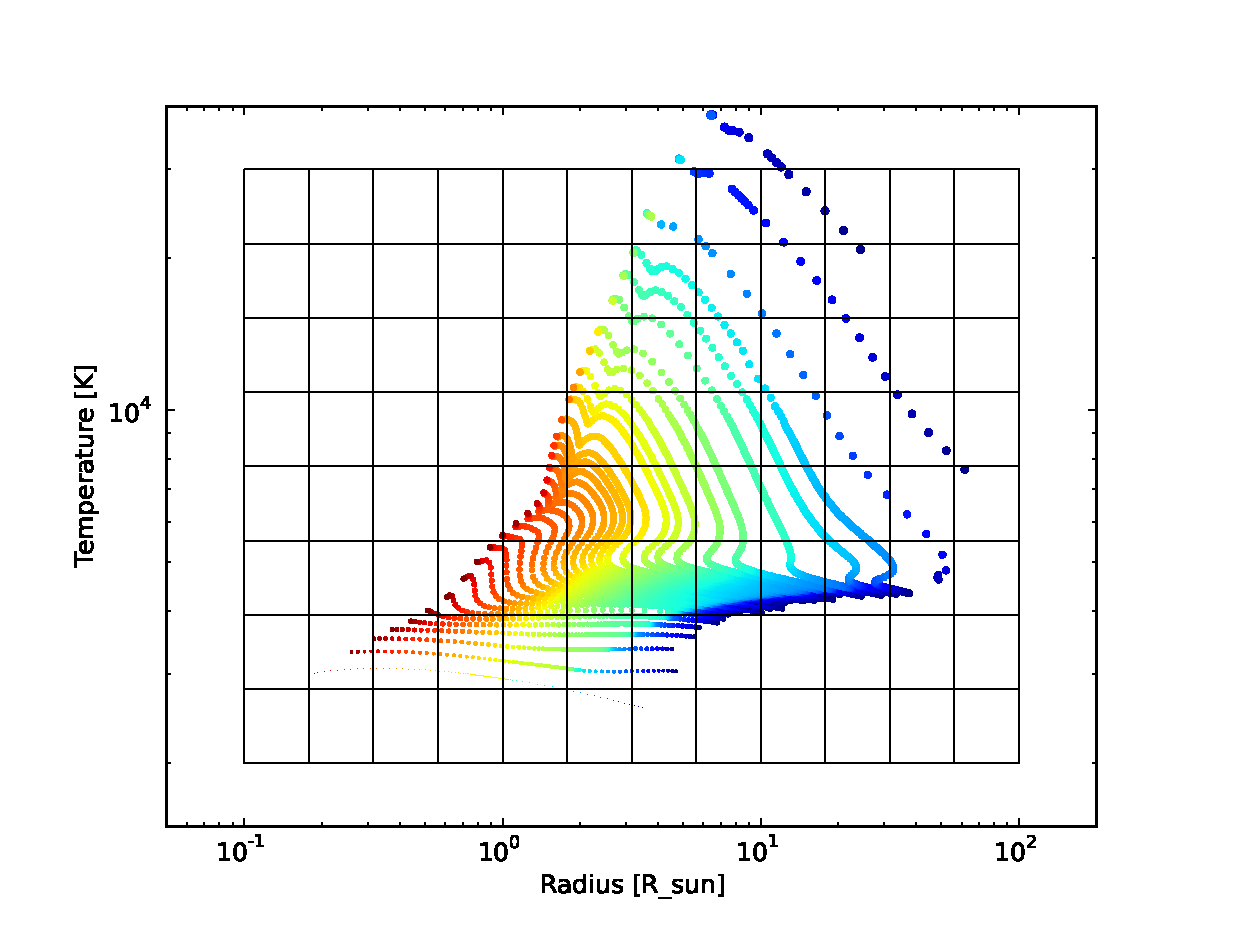
\includegraphics[width=3in]{temperature_vs_radius.eps}
\end{center}

While it would be nice to define the stellar properties in terms of $\lstar$ and $\tstar$, $\lstar$ depends strongly on $\tstar$ (fourth power), so that all the pre-main-sequence tracks lie in a narrow diagonal range in a ($\lstar$, $\tstar$) diagram. Therefore, if one samples a uniform grid in these two parameters, most models are wasted in unphysical regions. Instead, we should define the grid in terms of $\tstar$ and $\rstar$, since these parameters are not as strongly correlated. The following figure shows the evolutionary tracks, and the proposed parameter space coverage. According to the tracks shown, a fraction of the models are still 'unphysical', but this is worth the unbiased coverage. The proposed coverage also goes to cooler and smaller objects than the current tracks include.

For temperatures including and above 4,000\,K, we use the Castelli and Kurucz photosphere models. Since we are not defining the star in terms of mass, we can't calculate the surface gravity. However, the surface gravity doesn't have a large impact on stellar photospheres below 20,000\,K, and even above it's only a 5-10\% effect, relative to the log[g]=4.0 models. So above 4,000\,K we use Castelli and Kurucz for log[g]=4.0. For temperatures below 4,000\,K, we can use the new GAIA grid, which is computed with the PHOENIX code. Below 3,000\,K surface gravity seems to matter, up to a 10-15\% level. This is probably going to mostly affect the near-infrared fluxes. For these, we also use log[g]=4.0 models.

\end{itemize}
         
\subsection{Disk}

The type of disk component is indicated by the \textbf{second} letter of the set name:

\begin{itemize}

\item[\textbf{--}] No disk

\item[\textbf{P}] Flared parametrized disk. This is a passive disk with no accretion luminosity and a density distribution given by:
$$
\rho(R,z,\phi) = \rho_0^{\rm disk}\,\left(\frac{R_0}{R}\right)^{\beta - p}\,\exp{\left[-\frac{1}{2}\left(\frac{z}{h(R)}\right)^2\right]}
$$
where the disk scaleheight $h(R)$ is given by:
$$
h(R) = h_0\,\left(\frac{R}{R_0}\right)^\beta
$$
$\rho_0^{\rm disk}$ is set by the total disk mass $M_{\rm disk}$. The density is set to zero outside $\rmaxd$. The parameters added to the model are:

\begin{center}
  \begin{tabular}{llp{4in}}
    \texttt{disk.mass} & $\mdisk$ & Sampled in log space between $10^{-8}$ and $0.1$\,$\msun$ [dust] \\
    \texttt{disk.rmax} & $\rmaxd$ & Sampled in log space between 50 and 5000\,AU \\
    \texttt{disk.beta} & $\beta$ & Sampled in linear space between 1.0 and 1.3 \\
    \texttt{disk.p} & $p$ & Sampled in linear space between -2.0 and 0.0 \\
    \texttt{disk.h100} & $h_0$ ($R_0=100$\,AU) & Sampled in log space between 1 and 20\,AU \\
  \end{tabular}
\end{center}

\item[\textbf{A}] Alpha accretion disk. To be defined.

\end{itemize}

\subsection{Envelope}

The type of envelope component is indicated by the \textbf{third} letter of the set name:

\begin{itemize}

\item[\textbf{--}] No envelope

\item[\textbf{P}] Power-law envelope. This is a simple spherically symmetric envelope with a density given by:
$$
\rho(r) = \rho_0^{\rm env}\,\left(\frac{r}{r_0}\right)^\gamma
$$
The parameters added to the model are:

\begin{center}
  \begin{tabular}{llp{4in}}
    \texttt{envelope.rho0} & $\rho_0^{\rm env}$ ($r_0=1000$\,AU) & Sampled in log space between $10^{-24}$\,g/cm$^3$ and $10^{-16}$\,g/cm$^3$ [dust]\\
     \texttt{envelope.power} & $\gamma$ & Sampled in linear space between -1.0 and -2.0 \\
  \end{tabular}
\end{center}

The envelope goes out to a radius determined by the density and temperature of the ambient medium.

\item[\textbf{U}] Ulrich envelope. This is the collapse model derived by Ulrich (1976). The density is given by:
$$
\rho(r,\theta) = \frac{\mdote}{4\pi\left(G\mstar\rc^3\right)^{1/2}}\left(\frac{r}{\rc}\right)^{-3/2}\left(1 + \frac{\mu}{\mu_0}\right)^{-1/2}\left(\frac{\mu}{\mu_0} + \frac{2\mu_0^2\rc}{r}\right)^{-1} = \rho_0^{\rm env}\left(\frac{r}{\rc}\right)^{-3/2}\left(1 + \frac{\mu}{\mu_0}\right)^{-1/2}\left(\frac{\mu}{\mu_0} + \frac{2\mu_0^2\rc}{r}\right)^{-1}
$$
where $\mu_0$ is given by the equation for the streamline:
$$
\mu_0^3 + \mu_0\left(\frac{r}{\rc} - 1\right) - \mu\left(\frac{r}{\rc}\right) = 0
$$
The parameters added to the model are:

\begin{center}
  \begin{tabular}{llp{4in}}
    \texttt{envelope.rho0} & $\rho_0^{\rm env}$ & Sampled in log space between $10^{-24}$ and $10^{-16}$\,g/cm$^3$ [dust] \\
    \texttt{envelope.rc} & $\rc$ & Sampled in log space between 50 and 5000\,AU (same as disk radius if present)  \\
  \end{tabular}
\end{center}

The envelope goes out to a radius determined by the density and temperature of the ambient medium. The range of values for 
$\rho_0^{\rm env}$ was found by running a Monte-Carlo simulation of the values of $\rho_0^{\rm env}$ for $\rc$ in the range 50 to 5000\,AU, $\mstar$ in the range 0.1 to 50\,$\msun$, and $\mdote$ in the range $10^{-8}$ to $10^{-3}$\,$\msun$/yr.

\item[\textbf{T}] Terebey/Shu/Cassen envelope. To be defined in future.

\end{itemize}

\subsection{Cavities}

The type of cavity component is indicated by the \textbf{fourth} letter of the set name:

\begin{itemize}

\item[\textbf{--}] No bipolar cavity
\item[\textbf{B}] Bipolar power-law cavity

This component can only be present if an envelope component is also present. The power-law cavity is defined as a region with boundary given by:
$$
z(R) = \left(\frac{R}{R_0}\right)^c
$$
For $|z| > z(R)$, the density is set to $\rho_0^{\rm cav}$. The value of $R_0$ is set by defining the half-opening angle of the cavity $\theta_0$ at a radius of 10,000\,AU:

The parameters added to the model are:

\begin{center}
  \begin{tabular}{llp{4in}}
    \texttt{cavity.power} & $c$ & Sampled in linear space between 1.0 and 2.0 \\
    \texttt{cavity.theta0} & $\theta_0$ & Sampled in linear space between 0. and 60. \\
    \texttt{cavity.rho0} & $\rho_0^{\rm cav} $ & Sampled in log space between the ambient density and $10^{-20}$\,g/cm$^3$ [dust]\\
  \end{tabular}
\end{center}

\end{itemize}

\subsection{Inner radii}

How the inner radius is set is indicated by the \textbf{fifth} letter of the set name

\begin{itemize}

\item[\textbf{S}] Inner holes of the disk and envelope, if present, are set to the dust sublimation radius. The dust sublimation radius is set to $r_{\rm sub} = r_{\rm thin}(T_{\rm sub})$ where $T_{\rm sub}=1,600$\,K.

The parameters added to the model are, where applicable:

\begin{center}
  \begin{tabular}{llp{4in}}
    \texttt{disk.rmin} & $\rmind$ & Fixed to $r_{\rm sub}$ \\
    \texttt{envelope.rmin} & $\rmine$ & Fixed to $r_{\rm sub}$ \\
  \end{tabular}
\end{center}

\item[\textbf{H}] Inner holes of the disk and envelope, if present, can be larger than the dust sublimation radius. The inner radii are expressed as multiples of the dust sublimation radius $r_{\rm sub} = r_{\rm thin}(T_{\rm sub})$ where $T_{\rm sub}=1,600$\,K.

The parameters added to the model are, where applicable:

\begin{center}
  \begin{tabular}{llp{4in}}
    \texttt{disk.rmin} & $\rmind$ & Sampled in log space between $r_{\rm sub}$ and $1000\,r_{\rm sub}$ \\
    \texttt{envelope.rmin} & $\rmine$ & Set to the same value as \texttt{disk.rmin} \\
  \end{tabular}
\end{center}

\end{itemize}

\subsection{Ambient medium}

The type of ambient medium is indicated by the \textbf{sixth} letter of the set name:

\begin{itemize}

\item[\textbf{--}] No ambient medium. This can only be done if there is no envelope.

\item[\textbf{M}] Typical ambient medium ($T_{\rm amb}=10$\,K, $\rho_{\rm amb}\approx10^2$/cm$^3$) included. The parameters added to the model are:

\begin{center}
  \begin{tabular}{llp{4in}}
    \texttt{ambient.temperature} & $T_{\rm amb}$ & Set to 10\,K \\
    \texttt{ambient.density} & $\rho_{\rm amb}$ & Set to $10^{-23}$\,g/cm$^3$ [dust] \\
  \end{tabular}
\end{center}

\end{itemize}

\subsection{Dust}

The type of dust is indicated by the \textbf{seventh} letter of the set name:

\begin{itemize}

\item[\textbf{I}] Typical ISM dust for star formation regions. Since the aim of this grid is to be a starting point for modeling (rather than the ultimate goal), it would make sense to at least compute all the models with ISM-like dust. We use the Weingartner \& Draine (2001) $R_{\rm V}=5.5$ case A Milky-Way dust with C/H = 30ppm, recomputed with the Draine (2003a,b) dielectric functions and abundances. \textbf{[Can't use the one from the website because it doesn't have the maximum linear polarization, so need to use own, but it disagrees a little with the one Bruce Draine has on his website. Have emailed Bruce Draine to ask if he has the full phase functions.]}
%Define this as a dust type with $a_{\rm min}=0.002$\,$\mu$m, $a_{\rm max}=1$\,$\mu$m, and a power-law distribution with power $p=-3.5$. The composition should be astronomical silicates and carbon in solar abundances, and should not include PAHs.

\item[\textbf{G}] Grain growth and settling. To be determined.

%We can then define a second dust type which is the same as the first, but with $a_{\rm max}=1$\,mm. This can be used in the disk to mimic the grain growth. Finally, in future, we can add PAH emission to all models by extrapolating the size distributions down to very small sizes, but this should not be in the initial models.
%     Adds: \texttt{disk.eta}
%     Sets: \texttt{disk.dust.amax} to 1000 microns

% Ossenkopf and Henning

\end{itemize}

\subsection{PAHs/VSGs}

The PAH/VSG properties are indicated by the \textbf{eighth} letter of the set name:

\begin{itemize}

\item[\textbf{--}] No PAHs/VSGs included

\item[\textbf{P}] PAHs/VSGs included. To be determined.
      
\end{itemize}

\section{Number of models}

The number of models should be a function of the true number of independent parameters (exclude fixed and linked parameters).

\section{Parameters}

\subsection{Grid resolution}

We use a spherical polar grid. For 1D models, use 400 radial cells. For 2D models, use 400 radial cells and 300 polar cells.

\subsection{Grid extent}

We only compute models with envelopes if there is also an ambient medium (power-law envelopes to infinity don't make sense). For disk models and models with only the central source, compute both with and without an ambient medium.

For disk models, in the absence of an ambient cloud medium, the grid outer radius is set to the disk outer radius. For stellar models, in the absence of an ambient cloud medium, the grid outer radius is set to 2\,$R_\star$.

For models that do assume an ambient cloud medium, the grid outer radius is set by the radius at which the optically thin temperature of dust would reach the ambient temperature of the cloud, or the radius at which the density in the envelope (if present) reaches the density of the ambient density of the cloud $\rho_0$, or the disk radius (if present), whichever is larger. Any densities lower than the ambient density are set to the ambient density (except inside $R_{\rm sub}$). In any case, the outer radii are then increased by a factor of $\sqrt{2}$ so as to be able to do the radiation transfer in a slab that includes all of the medium at temperatures hotter than the ambient medium.

\subsection{Minimum temperature}

The minimum temperature of any dust should be set to 2.725K in the absence of an ambient medium, or to the ambient temperature if an ambient medium is present.

\subsection{Raytracing}

We use raytracing for the source and dust thermal emission.

\subsection{Number of photons}

We choose $1,000,000$ photons for the temperature calculation, for the image/SED iteration, and for the raytracing. For 1D models, we use 1,000 photons for each temperature iteration.

\subsection{Viewing angles}

For 1D models, we use a single viewing angle at ($45^\circ$, $45^\circ$). For 2D models, we sample 10 viewing angles between $i=0^\circ$ and $i=90^\circ$ (no $\cos(i)$ sampling). Correcting the bias in fitting results should be simple using weighting.

\subsection{Apertures}

Define apertures in units of $r_{\rm thin}(T_d)$, or more generally $\rmine$/$\rmind$ and $\rmaxe$/$\rmaxd$, to optimize information gained from the models. Fitting is easier with absolute apertures that are always the same, but we can always pre-interpolate convolved fluxes to the absolute apertures later on. Define 10 apertures spaced logarithmically between the minimum and maximum radii. Since $\rmaxe/\rmine$ is typically around $10^6$ this is a little more than one aperture per order of magnitude size-scale.

\subsection{MRW and PDA}

We should definitely use the MRW and PDA. For the MRW, $\gamma=2$ is sensible with the caveat that the temperatures may not be as accurate as the SEDs.

\subsection{Temperature iterations}

We can specify the convergence criteria to:

\begin{itemize}
\item Percentile = 99\%
\item Absolute threshold = 2
\item Relative threshold = 1.1
\end{itemize}

and we set the maximum number of iterations to 10.

\subsection{Dust destruction}

Issue with using dust destruction is that the parameters that describe the disk are then not really correct. For example if the disk is enlarged by dust destruction then the inner radius is not really right. In spherical envelopes with no cavities, this might matter because the inner radius can be a bit larger due to the radiation bouncing around in the inner hole. But if we don't do it, some models might take a long time to run. Could always flag models where a significant amount of dust is destroyed so people know to be cautious. Anyway, we are using dust destruction to specify the inner radius so doesn't make too much sense to only go there halfway and destroy it analytically but not numerically.

Clearly indicate that $R_{\rm sub}$ is not necessarily true sublimation radius, but just the radius where the optically thin temperature would fall to $T_{\rm sub}$

\section{Output}

This section discusses what we should output from the grid, and how much storage is expected for each element.

\subsection{SEDs}

We can compute SEDs from $10^{-2}$ to $10^4$\,$\mu$m for 250 wavelengths (need to go that low because of the x-rays, unless we can just capture how much flux falls outside the SED range?). We should save I, Q, U, V. These need to be saved in 64-bit floating point numbers, as the fluxes can be quite large and cause 32-bit overflow. Save polarization I, Q, U, and V. Save uncertainties on the values. Track photon origin. A lot of SED values are going to be zero, but that should be taken care of by the compression, so won't affect storage.

\subsection{Images}

SEDs are best computed using 'binned' SEDs in wavelength, but images are best computed using the monochromatic wavelength feature. Therefore it makes sense to initially only compute SEDs, and then once it is 'complete', we can start computing images can be computed in post processing using the monochromatic wavelength feature of the code. They also take up quite a bit of disk space, so we first need to see how large the SED grid will be.

\subsection{Grids}

We should probably save all the quantities in 32-bit floating point to save storage space.

Keep \texttt{specific\_energy\_abs} in last iteration. Can compute temperature on the fly from \texttt{\texttt{specific\_energy\_abs}} given the dust properties. This should actually be quite easy because the \texttt{specific\_energy\_abs} is derived from the temperature which has already had minimum/maximum values applies to it.

Also keep density difference in last iteration, to keep track of dust destroyed.

\subsection{Compression}

Ensure that all output is compressed to maximum level.

\subsection{Caveats}

\begin{itemize}

\item The stellar photospheres used are for a fixed surface gravity of log[g] = 4.0. This mostly affects the molecular bands in the near-infrared for cool stars, at the 10\% level.

\item The outer envelope radii do not take into account that scattered light might be seen out to larger radii, but there is no way to know that in advance, so will have to go through the results and check the extent of the scattered light (which can be done because we will have the separated components for the SEDs).

\item The modified random walk is used with $\gamma=2$ which means that while the SEDs will be accurate enough, the temperatures may be slightly different compared to the exact solution (see Min et al., 2009)

\item For models that take into account accretion, the gas emission is not included inside the dust sublimation radius. If the gas is optically thin, then the emission is mostly in lines, but this might mean that the results are inaccurate for optically thick gas. In addition, for embedded sources, since the line emission will get reprocessed, this could lead to an underestimated luminosity overall.

\item When we select only photons from the slab, material outside the slab might still contribute to the extinction - but in most cases this is not likely to be important.

\end{itemize}

\section{Bonuses}

\begin{itemize}

\item The stellar parameters do not rely on evolutionary tracks

\end{itemize}

\section{Optimizations}

\begin{itemize}
\item For power-law envelopes only with no cavities, can use 1D grid and fewer photons for temperature and only need one viewing angle for SEDs.
\end{itemize}

\end{document}
